\documentclass{beamer}

\usepackage[english]{babel}
\usepackage[utf8]{inputenc}
\usepackage[T1]{fontenc}
\usepackage{tikz}

\usetheme{nescala}
\setbeamercovered{transparent}

\newcommand\demoslide{
  {
    \setbeamertemplate{background}{}
    \begin{frame}[plain]
      \begin{center}\Large\bfseries Demo\end{center}
    \end{frame}
  }
}

\newcommand\fullpicture[1]{
  {
    \setbeamertemplate{background}{}
    \begin{frame}[plain]
      \begin{tikzpicture}[remember picture,overlay]
        \node[at=(current page.center)] {
          \includegraphics[keepaspectratio,height=1.2\paperheight,width=1.2\paperwidth]{#1}
        };
      \end{tikzpicture}
    \end{frame}
  }
}

\begin{document}

  \title{Macros vs Types}
  \author{Eugene Burmako \& Lars Hupel}
  \institute{\'Ecole Polytechnique F\'ed\'erale de Lausanne\\Technische Universit\"at M\"unchen}
  \date{March 1, 2014}

{
\setbeamertemplate{footline}{}
\begin{frame}
  \titlepage
\end{frame}
}

\begin{frame}
\vskip40pt
\begin{center}
\text{\color{blue}{\Large{Static checks}}}
\end{center}
\end{frame}

\begin{frame}{Types \'a la Pierce}
  \begin{quote}
    ``A type system is a tractable syntactic method for \alert<2>{proving the absence of certain program behaviors} by classifying phrases according to the kinds of values they compute.''
  \end{quote}
  \hfill -- Benjamin Pierce, in: Types and Programming Languages
\end{frame}

\begin{frame}{Types \'a la Scala}
  Scala has a sophisticated type system
  \begin{itemize}
    \item path-dependent types
    \item type projections
    \item higher-kinded types
    \item implicits
  \end{itemize}
\end{frame}

\begin{frame}{Type computations}
  implicits allow computations in the type system

  \begin{itemize}
    \item higher-order unification (SI-2712)
    \item generic operations on tuples
    \item extensible records
    \item statically size-checked collections
  \end{itemize}
\end{frame}

\begin{frame}[fragile]{Type Computations}{Example: Sized collections}
  \begin{verbatim}
// typed as Sized[_2, List[String]]
val hdrs = Sized("Title", "Author")

// typed as List[Sized[_2, List[String]]]
val rows = List(
  Sized("TAPL", "B. Pierce"),
  Sized("Implementation of FP Languages", "SPJ")
)
  \end{verbatim}
\end{frame}

\demoslide

\begin{frame}{The Power of Type Computation}
  Computing with implicits is sometimes called ``Poor Man's Prolog''
  \vspace{1em}

  But: Almost anything can be done
\end{frame}

% <https://secure.flickr.com/photos/mszeto/3261725397/>
\fullpicture{img/hanoi.jpg}

\begin{frame}{How Can Macros Help?}
  \begin{itemize}
    \item type system covers many properties
    \item complex type computations are hard to debug

      (sometimes, \texttt{-Xlog-implicits} is not enough)
    \item implicit-heavy code slows down compiler significantly
    \item our advice:
      \begin{itemize}
        \item types whenever possible
        \item macros when it becomes too heavyweight
      \end{itemize}
  \end{itemize}
\end{frame}

\begin{frame}[fragile]{Use Case: Checked Arithmetics}
  Spire provides a \texttt{checked} macro to detect arithmetic overflows

  \vspace{1em}
  \begin{verbatim}
// returns None when x + y overflows
Checked.option {
  x + y < z
}
  \end{verbatim}
\end{frame}

\begin{frame}
\vskip40pt
\begin{center}
\text{\color{blue}{\Large{Code generation}}}
\end{center}
\end{frame}

\begin{frame}[fragile]{(Textual) Code Generation}{Example: Parser Generators}
  % from Tom Niemann <epaperpress.com>
  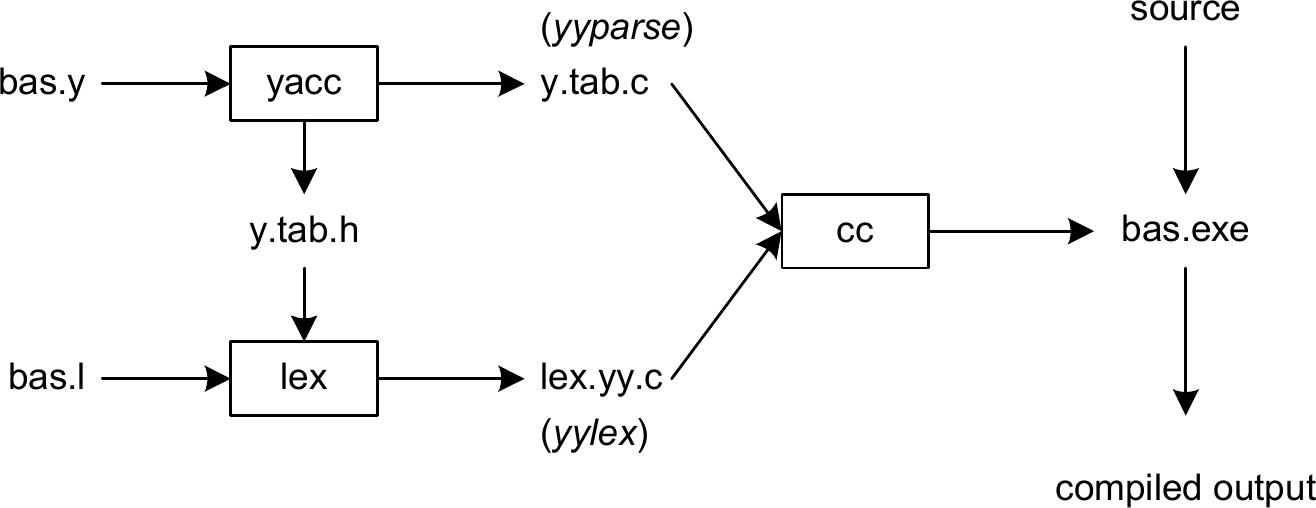
\includegraphics[width=\linewidth]{img/yacc.png}
\end{frame}

\begin{frame}{Code Generation}
  Almost every language has it\only<1>{.}\visible<2->{, even Haskell:}

  \begin{visibleenv}<2->
    \begin{itemize}
      \item \texttt{lens}

         derive lenses for fields of a data type
      \item \texttt{yesod}

        templating, routing
      \item \texttt{invertible-syntax}

        constructing partial isomorphisms for constructors

      \item ... more examples in the TH paper
    \end{itemize}
  \end{visibleenv}
\end{frame}

\begin{frame}{Type Classes in Scala}
  \begin{itemize}
    \item type classes are (first-class) traits
    \item instances are (first-class) values
    \item<visible@2> both can use arbitrary language features
  \end{itemize}
\end{frame}

\begin{frame}{Use Case: Materialization}
  We want to have: default instances for type classes
  \begin{itemize}
    \item \texttt{Semigroup} (pointwise addition)
    \item \texttt{Ordering} (lexicographic order)
    \item \texttt{Binary} (pickling/unpickling)
  \end{itemize}

  \vspace{1em}
  We do not want to: write boilerplate
  \begin{itemize}
    \item repetitive \& error-prone
  \end{itemize}
\end{frame}

\begin{frame}{Use Case: Materialization}
  \texttt{scalac} already synthesizes \texttt{equals}, \texttt{toString} ...

  \vspace{1em}
  \begin{alertblock}{Problem}
    not based on Type Classes
  \end{alertblock}

  \vspace{1em}
  \begin{exampleblock}{Solution}
    materialization based on implicit macros
  \end{exampleblock}
\end{frame}

\begin{frame}[fragile]{Use Case: Materialization}
  \begin{verbatim}
implicit def derive[C[_] : TypeClass, T]: C[T] =
  macro TypeClass.derive_impl[C, T]
  \end{verbatim}
\end{frame}

\demoslide

\begin{frame}{The Power of Materialization}
  \begin{itemize}
    \item similar to \texttt{deriving Eq} in Haskell
    \item extensible without modifying the macro(s) itself
  \end{itemize}
\end{frame}

\begin{frame}[fragile]{The Dangers of Materialization}
  Whitebox macros allow us to write this:
  \vspace{1em}

  \begin{verbatim}
implicit def deriveAnything: Any =
  macro derive_impl
  \end{verbatim}
\end{frame}

\begin{frame}{Macros and Code Generation}
  \begin{block}{Advice}
    \begin{itemize}
      \item don't abandon typing discipline
      \item prefer vanilla Scala
      \item try to encapsulate only the ``moving parts'' into a macro

        (maybe more boilerplate, but more predictable)
      \item try to constrain the types of the macros as much as possible
    \end{itemize}
  \end{block}
  \vspace{1em}

  \begin{block}{Open Problems}
    Best practices for documentation \& testing
    \vspace{1em}

    Do we need a compile-time ScalaCheck?
  \end{block}
\end{frame}

\begin{frame}
\vskip40pt
\begin{center}
\text{\color{blue}{\Large{Domain-specific languages}}}
\end{center}
\end{frame}

\begin{frame}
\vskip40pt
\begin{center}
\text{\color{blue}{\Large{Summary}}}
\end{center}
\end{frame}

\end{document}
